\documentclass{article}

% ----------------Report particulars --------------------%
\title{Remote Sensing Notes} 
\author{Rosa Trancoso}
\date{\today\\v0.1}


% Usual latex stuff
%----------- Load user packages (optional) --------------%

% Language and font encodings
\usepackage[english]{babel}
\usepackage[utf8x]{inputenc}
\usepackage[T1]{fontenc}

% \usepackage[scaled]{uarial}
\renewcommand{\familydefault}{\sfdefault}

% Sets page size and margins
\usepackage{parskip}

\usepackage{amsmath}
\usepackage[pdftex]{graphicx}
\usepackage{placeins} % FloatBarrier

\usepackage{acro}  % printacronyms

\usepackage[a4paper]{geometry} % textwidth 418pt (14cm) instead of 345pt (12...cm)

% % other
% \usepackage[colorinlistoftodos]{todonotes}
\usepackage[colorlinks=true, allcolors=blue]{hyperref}
\usepackage{soul} % hl

% \usepackage{subcaption}
% \usepackage{natbib}
\usepackage{url}
\usepackage{tabulary}
\usepackage{booktabs} % toprule
% \usepackage{tabto}
% \usepackage[]{dirtree}
% \usepackage{multimedia}
% \usepackage{pdfpages}
\usepackage{longtable}

\usepackage{xspace}

\usepackage{layouts} % \printinunitsof{cm}\prntlen{\textwidth}


%-------------- Definitions (optional) -----------------%

\def\deg{$^\circ$\xspace}
\def\ms{m s\textsuperscript{-1}\xspace}

\DeclareAcronym{ec}{short=EC,long=European Commission} 
\DeclareAcronym{esa}{short=ESA,long=European Space Agency}
\DeclareAcronym{geoss}{short=GEOSS,long=Global Earth Observation System of Systems}
\DeclareAcronym{gmes}{short=GMES,long=Global Monitoring for Environment and Security programme}
\DeclareAcronym{isar}{short=ISAR,long=Inverse Synthetic Aperture Radar}
\DeclareAcronym{miras}{short=MIRAS,long=Microwave Imaging Radiometer using Aperture Synthesis}
\DeclareAcronym{mtg}{short=MTG,long=Meteosat Third Generation}
\DeclareAcronym{mtg-s}{short=MTG-S,long=Meteosat Third Generation-Sounder}
\DeclareAcronym{sar}{short=SAR,long=Synthetic Aperture Radar}
\DeclareAcronym{smos}{short=SMOS,long=Soil Moisture Ocean Salinity}

\DeclareAcronym{agri}{short=AGRI,long=Advanced Geosynchronous Radiation Imager}
\DeclareAcronym{fd}{short=FD,long=Full Disk}
\DeclareAcronym{vissr}{short=VISSR,long=Visible and Infrared Spin-Scan Radiometer}
\DeclareAcronym{giirs}{short=GIIRS,long=Geostationary Interferometric Infrared Sounder}
\DeclareAcronym{lmi}{short=LMI,long=Ligthning Mapping Imager}
\DeclareAcronym{sep}{short=SEP,long=Space Environment Package}
\DeclareAcronym{sem}{short=SEM,long=Space Environment Monitor}
\DeclareAcronym{cma}{short=CMA,long=China Meteorological Administration}
\DeclareAcronym{cast}{short=CAST,long=China Academy of Space Technology}


% \DeclareAcronym{cfsr}{short=CFSR,long=Climate Forecast System Reanalysis}
% \DeclareAcronym{ncep}{short=NCEP,long=National Centers for Enviromental Prediction}
% \DeclareAcronym{nhc}{short=NHC,long=National Hurricane Center}
% \DeclareAcronym{sst}{short=SST,long=Sea Surface Temperature}
% \DeclareAcronym{st2}{short=ST2,long=\citet{short=,long=short=hereafter ST2,long=Tolman:1996}}


% --------------- Beginning Document --------------------%
\begin{document}
\maketitle

\begin{abstract}
the abstract should have 6 sentences. 1. Topic 2. Importance 3. Here we

textwidth in pt: \the\textwidth

textwidth in cm: \printinunitsof{cm}\prntlen{\textwidth}
 
\end{abstract}

\tableofcontents

% ------------------------------------------
% Introduction
% ------------------------------------------
\section{Introduction}
\label{sec:intro}


Remote sensing is the scanning of the earth by satellite or high-flying aircraft in order to obtain information about it.
Remote sensing is the acquisition of information about an object or phenomenon without making physical contact with the object and thus in contrast to on-site observation\footnote{\url{https://en.wikipedia.org/wiki/Remote_sensing}}.

Remote sensors can be either passive or active. Passive sensors respond to external stimuli. They record natural energy that is reflected or emitted from the Earth's surface. The most common source of radiation detected by passive sensors is reflected sunlight. In contrast, active sensors use internal stimuli to collect data about Earth. For example, a laser-beam remote sensing system projects a laser onto the surface of Earth and measures the time that it takes for the laser to reflect back to its sensor\footnote{\url{http://oceanservice.noaa.gov/facts/remotesensing.html}}.

Examples of passive remote sensors include film photography, infrared, charge-coupled devices, and radiometers (wiki)
Examples of active remote sensors are Radar and Lidar where the time delay between emission and return is measured, establishing the location, speed and direction of an object (wiki).

The quality of remote sensing data consists of its spatial, spectral, radiometric and temporal resolutions.

\subsection{Active Sensors}
\subsubsection{Radar}
Radar is an object-detection system that uses radio waves to determine the range, angle, or velocity of objects. The radar signals that are reflected back towards the transmitter are the desirable ones that make radar work. If the object is moving either toward or away from the transmitter, there is a slight equivalent change in the frequency of the radio waves, caused by the Doppler effect. 
Radar signals are reflected especially well by materials of considerable electrical conductivity—especially by most metals, by seawater and by wet ground. Some of these make the use of radar altimeters possible.
\footnote{\url{https://en.wikipedia.org/wiki/Radar}}

\begin{table}[h!]
\centering
\label{fig:radar_bands}
\caption{Radar Frequency Bands. Source: \url{https://en.wikipedia.org/wiki/Radar}}
% \begin{tabulary}{\textwidth}{p{1cm}p{2cm}p{2cm}L}
\begin{tabulary}{\textwidth}{LLLL}
\toprule
\parbox{5em}{Name} & \parbox{10em}{Frequency} & \parbox{10em}{Wavelength} & Notes \\ 
\midrule
HF & 3-30 MHz & 10-100 m & Coastal radar systems; "High Frequency" \\
VHF & 30-300 MHz & 1-10 m & Very long range, ground penetrating; "Very High Frequency" \\
... &  & & \\
S & 2-4 GHz & 7.5-15 cm & Moderate range surveillance; Terminal air traffic control; long-range weather; marine radar; "Short" \\
C & 4-8 GHz & 3.75-7.5 cm & Satellite transponders; a "Compromise" between X and S bands; weather; long-range tracking \\
X & 8-12 GHz & 2.5-3.75 cm & Missile guidance; marine radar; weather; medium-res mapping and ground surveillance; names "X" because it was secret during WW2 \\
... &  & & \\
\bottomrule
\end{tabulary}
\end{table}

Radar Imaging is an application of radar which is used to create two-dimensional images.\footnote{\url{https://en.wikipedia.org/wiki/Radar_imaging}}

Imaging radar has several advantages.[3] It can operate in the presence of obstacles that obscure the target, and can penetrate ground (sand), water, or walls.[4][5]

Current radar imaging techniques rely mainly on \ac{sar} and \ac{isar} imaging. Emerging technology utilizes monopulse radar 3-D imaging.


\paragraph{SAR}

\begin{table}[h!]
\label{fig:radar_bands}
\caption{Commercial Radar Remote Sensing Satellites. Source:\url{http://eijournal.com/print/articles/discover-the-benefits-of-radar-imaging}}
\begin{tabulary}{\textwidth}{p{2.1cm}p{1.5cm}p{1cm}p{1cm}p{1cm}LL}
\toprule
Satellite Mission & Launch Date & Band & Res [m] & Swath Width [km] & Repeat Date [days] & Description \\ 
\midrule
TerraSAR-X / TanDEM-X & 2007/2010 & X & 1-18 & 5-150 & 11 & German public-private mission \\
\midrule
COSMO-SkyMed & 2007/2008 & X & 1-100 & 10-200 & 16 & Italian constellation of four satellites \\
\midrule
RADARSAT-1 / RADARSAT-2 & 1995/2007 & C & 3-100 & 20-500 & 24 & Canadian commercial mission \\
\midrule
PAZ & 2013 & X & 1-18 & 5-150  & 11 & Spanish dual-use mission, constellation with TerraSAR-X and TanDEM-X envisioned \\ \bottomrule
\end{tabulary}
\end{table}



\subsubsection{Lidar}





% ------------------------------------------
\section{International Programmes}
\label{sec:intprog}
% ------------------------------------------

\subsection{Copernicus}
\label{ssec:copernicus}

Copernicus is the new name for the \ac{gmes} programme. 

This initiative is headed by the \ac{ec} in partnership with the \ac{esa}.

\ac{esa} coordinates the delivery of data from upwards of 30 satellites and the \ac{ec}, acting on behalf of the European Union, is responsible for the overall initiative, setting requirements and managing the services\footnote{\url{http://www.esa.int/Our_Activities/Observing_the_Earth/Copernicus/Overview3}}.

\ac{esa} is developing a new family of satellites, called Sentinels (section \ref{ssec:sentinels}) specifically for the operational needs of the Copernicus programme.

This programme is the European contribution to the worldwide \ac{geoss}.

The Copernicus Space Component comprises two types of satellite missions, ESA's families of dedicated Sentinels and missions from other space agencies, called Contributing Missions. A unified ground segment, through which the data are streamed and made freely available for Copernicus services, completes the Space Component.


% ------------------------------------------
% Introduction
% ------------------------------------------
\section{Satellites}
\label{sec:satellites}

\hl{optical, radar and altimetry}
\hl{geostationary, polar}
\hl{SAR}
\hl{multispectral}
\hl{sounder}

\subsection{FY-4}
\label{fy-4}

FY-4 is \ac{cma}'s second-generation three-axis stabilized, geostationary meteorological satellite series, under development by \ac{cast}. Two variants of spacecraft of the FY-4 (FenYun means "winds and clouds or storm" in Chinese) program are in planning, with one carrying optical sensors and the other carrying microwave sensors.

Compared to the current FY-2 geostationary meteorological satellite series, the performance of the FY-4 series has been considerably improved in terms of data amount, network transmission bandwidth, product type and quantity and archiving data and applications. The new generation FY-4 satellites are designed with an enhanced imagery scanning capability, desirable for monitoring small and medium scale weather systems. FY-4 is enabled with vertical atmospheric sounding and microwave detection capabilities to address 3D remote sensing at geostationary altitudes. The new FY-4 series is also enabled with solar observations for EUV (Extreme Ultraviolet) and X-ray monitoring, in a bid to enhance China's space weather watch and warning capability. 1)

Based on user requirements and technical feasibility, the missions of the FY-4 series include imagery, sounding, lightning mapping, and space environment monitoring. HRIT (High Rate Information Transmission), LRIT (Low Rate Information Transmission) data transmission, and DCP (Data Collection Platform) services are available for users. 2) 3) 4) 5)

In 2015, the Chinese government approved the NSIP (National Space Infrastructure Plan) covering also the meteorological program of LEO and GEO missions up to 2025. 6)


\begin{table}[h!]
\centering
\label{fig:fy4_vs_fy2}
\caption{The FY family. Source: \url{https://directory.eoportal.org/web/eoportal/satellite-missions/f/fy-4}}
\begin{tabulary}{\textwidth}{p{2cm}LL}
\toprule
Instrument & FY-4 & FY-2 \\ 
\midrule
Imaging &   \textbf{AGRI} (Advanced Geosynchronous Radiation Imager) (AGRI) \newline 
            14 channels \newline
            Spatial resolution: 0.5-4 km \newline
            \ac{fd} imaging: 15 min \newline 
            Rapid Scan: 2.5 min 
        &   \textbf{VISSR} (Visible and Infrared Spin-Scan Radiometer\newline
             5 channels \newline
            Spatial resolution: 1.25-5 km \newline
            \ac{fd} imaging: 30 min \newline
            Rapid Scan: 3-6 min \\
\midrule
Sounding & \textbf{GIIRS} (Geostationary Interferometric Infrared Sounder) \newline
            913 channels \newline
            Spectral resolution: 0.8 to 1.6 $cm^{-1}$ \newline
            Spatial resolution: 16 km 
        &  Not Applicable \\
\midrule
Lightning \newline 
Mapping &   \textbf{LMI} (Ligthning Mapping Imager) \newline   
            \hl{SSP} resolution: 7.8 km
        &  Not Applicable \\
\midrule
&   \textbf{SEP} (Space Environment Package) \newline
    High energy particles \newline
    Magnetic field: Solar X ray fluxes 
&   \textbf{SEM} (Space Environment Monitor) \newline
    High energy particles \\
\bottomrule
\end{tabulary}
\end{table}


\begin{figure}[h!]    
\centering
\label{fig:nz_probaV}
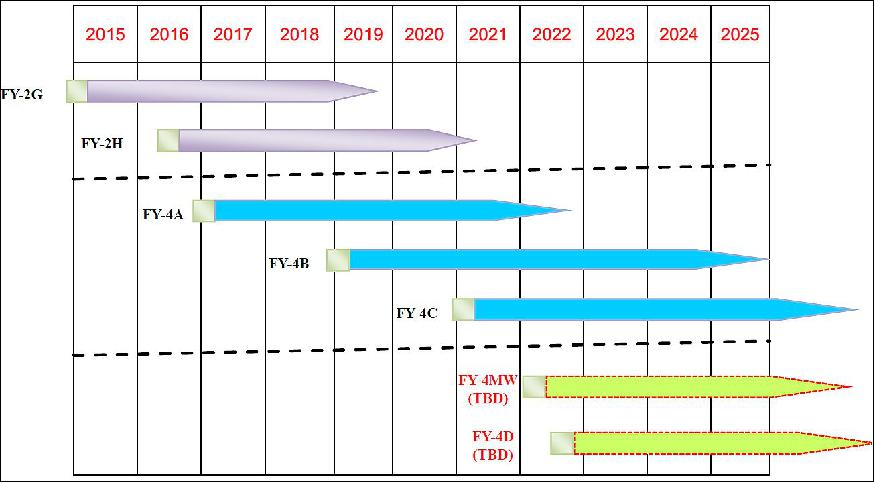
\includegraphics[width=\linewidth]{figures/FY4_Auto4.jpeg}
\caption{
Overview of the GEO meteorological launch program of CMA for the next decade (image credit: CMA, source: \url{https://directory.eoportal.org/web/eoportal/satellite-missions/f/fy-4}}
\end{figure}




\subsection{Proba-V}
\label{probaV}
Proba-V (V for Vegetation) is a ESA Miniature satellite (140 kg), launched in May 2013\footnote{\url{http://www.esa.int/Our_Activities/Space_Engineering_Technology/Proba_Missions/Overview2}}. 

It provides global coverage every two days, with latitudes 35-75\deg N and 35-56\deg S covered daily, and between 35\deg S and 35 \deg N  every 2 days. 
The Proba-V imager's continent-spanning 2250 km field of view collects light in the blue, red, near-infrared and mid-infrared wavebands, ideal for monitoring plant and forest growth as well as inland water bodies. The Vegetation instrument can distinguish between different land cover types and plant species, including crops, to reveal their health, as well as detect water bodies and vegetation burn scars.

The ESA Earth Watch Programme provides 1km data, which is complemented by a National Programme supplying products at 300m/600m resolution (available as ESA Third Party Mission)\footnote{\url{https://earth.esa.int/web/guest/missions/esa-operational-eo-missions/proba-v}}

The Proba-V image at 300 m resolution, acquired mid July 2016,takes a closer look at the South island of New Zealand (see Figure \ref{fig:nz_probaV}).

\begin{figure}[h!]    
\centering
\label{fig:nz_probaV}
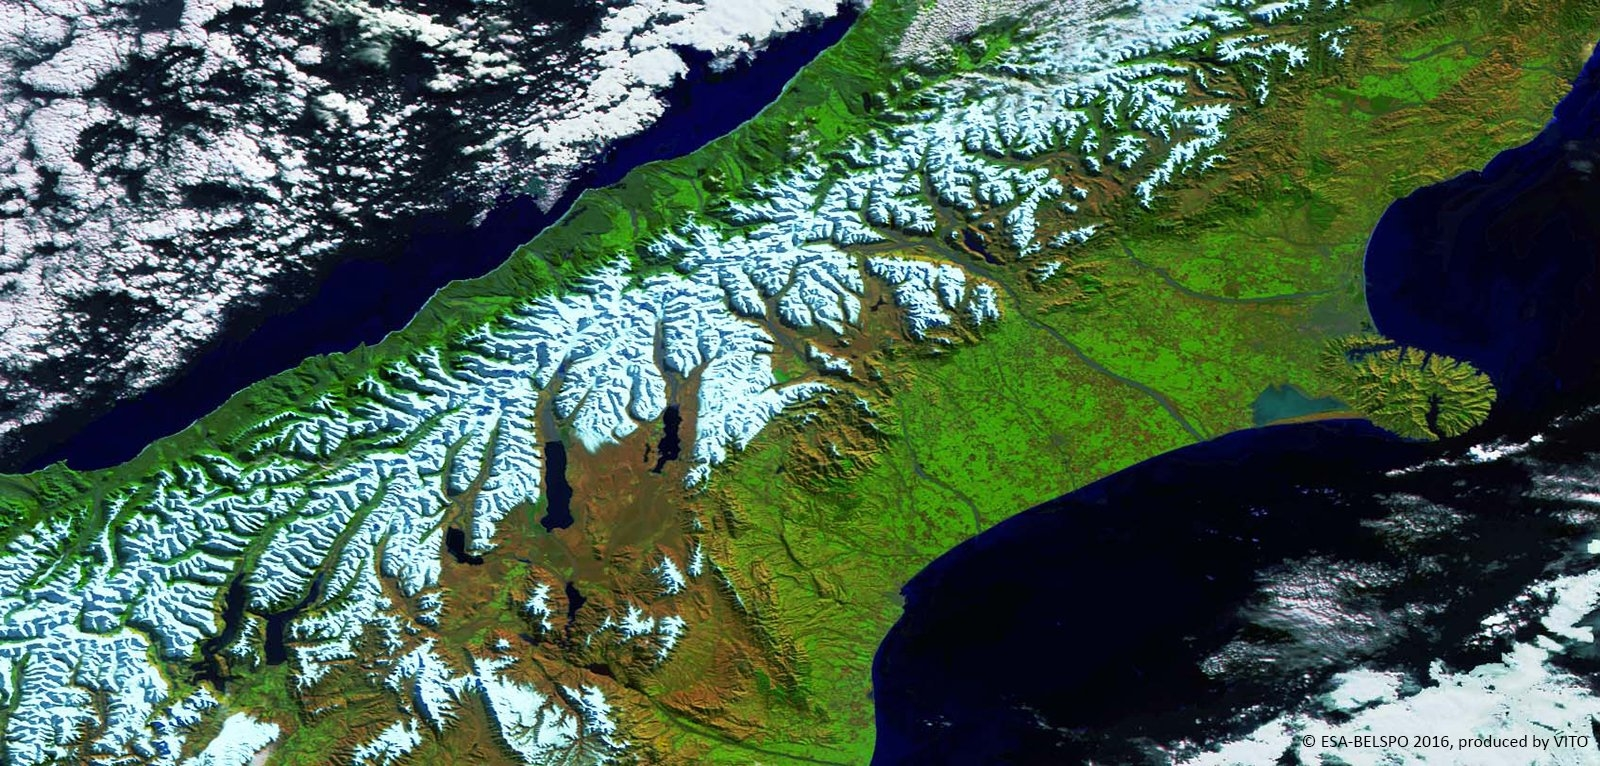
\includegraphics[width=\linewidth]{figures/New-Zealand_probaV.png}
\caption{South Island of New Zealand captured by Proba-V at 300 m resolution, mid July 2016
Source: \url{https://earth.esa.int/web/guest/missions/esa-operational-eo-missions/proba-v/image-of-the-week/-/article/new-zealand
}}
\end{figure}

\subsection{SMOS}

ESA's \ac{smos} Earth Explorer mission is a radio telescope in orbit, but pointing back to Earth not space. It's \ac{miras} radiometer picks up faint microwave emissions from Earth's surface to map levels of land soil moisture and ocean salinity. These are the key geophysical parameters, soil moisture for hydrology studies and salinity for enhanced understanding of ocean circulation, both vital for climate change models.\footnote{\url{https://earth.esa.int/web/guest/missions/esa-operational-eo-missions/smos}}


\subsection{Sentinels}
\label{ssec:sentinels}

The Sentinels are a family of satellites developed specifically for the operational needs of the Copernicus programme (see section \ref{ssec:copernicus}). 

Each Sentinel mission is based on a constellation of two satellites to fulfil revisit and coverage requirements. 

These missions carry a range of technologies, such as radar and multi-spectral imaging instruments for land, ocean and atmospheric monitoring:

\begin{itemize}

\item \textbf{Sentinel-1} is a polar-orbiting, all-weather, day and night radar mission for land and ocean services. Sentinel-1A and -1B were launched respectively in April 2014 and April 2016. Both were taken into orbit on a Soyuz rocket from Europe's Spaceport in French Guiana.

\item \textbf{Sentinel-2} is a polar-orbiting multispectral mission delivering high-resolution optical images for land services, for example, imagery of vegetation, soil and water cover, inland waterways and coastal areas. Sentinel-2 can also deliver information for emergency services. Sentinel-2A was launched on 23 June 2015 and Sentinel-2B followed on 7 March 2017. 

\item \textbf{Sentinel-3} is a multi-instrument mission that provides high-accuracy optical, radar and altimetry data for marine and land services, for example, sea surface height, sea and land surface temperature, ocean colour and land colour. The mission will support ocean forecasting systems, as well as environmental and climate monitoring. Sentinel-3A was launched on 16 February 2016. 

\item \textbf{Sentinel-4} is devoted to atmospheric composition monitoring and will be embarked upon a \ac{mtg-s} satellite in geostationary orbit. 

\item \textbf{Sentinel-5} will also provide data for atmospheric composition monitoring but from a polar orbit, aboard a MetOp Second Generation satellite.

\item \textbf{Sentinel-5 Precursor} mission is being developed to reduce data gaps between Envisat, in particular the Sciamachy instrument, and the launch of Sentinel-5. 

\item \textbf{Sentinel-6} will carry a radar altimeter to measure global sea surface height, primarily for operational oceanography and for climate studies. 

\end{itemize}

\begin{figure}[h!]    
\centering
\label{fig:sentinels}
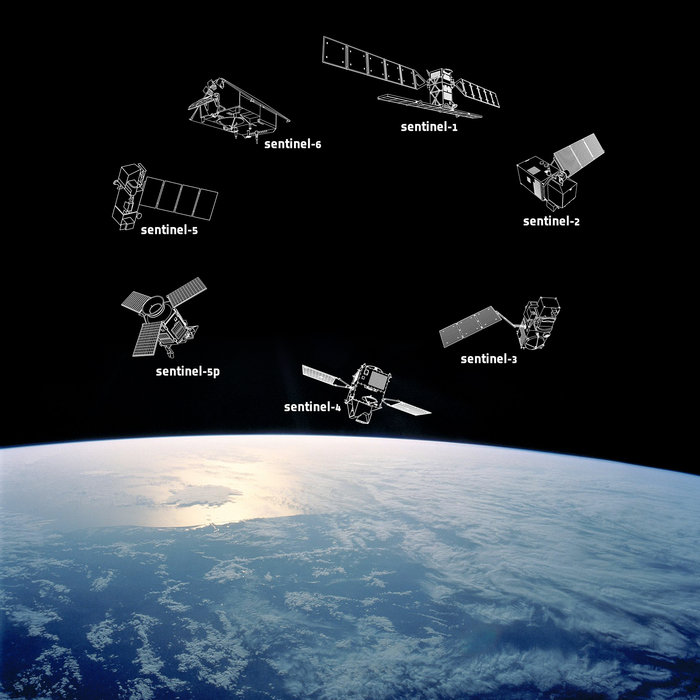
\includegraphics[width=0.5\linewidth]{figures/Sentinel_family_node_full_image_2.jpg}
\caption{The Sentinel family. Source: \url{http://www.esa.int/var/esa/storage/images/esa_multimedia/images/2014/04/sentinel_family/14493549-1-eng-GB/Sentinel_family_node_full_image_2.jpg}}
\end{figure}

\begin{table}[h!]
\centering
\label{fig:sentinels}
\caption{The Sentinel family.}
\begin{tabulary}{\textwidth}{p{1cm}p{1cm}LL}
\toprule
Sentinel & Orbit & Period & Description of Mission \\ 
\midrule
1 & Polar & 1-A: Apr 2014; 1-B: Apr 2016 & All weather, day and night radar \\
\midrule
2 & Polar & 2-A: Jun 2015; 2-B: Mar 2017 & Hi-res optical (multispectral) for land; Emergency services \\
\midrule
3 &       & 3-A: Feb 2016 & Multi-instrument: optical, radar and altimetry; Land and marine services: SSH, SST, LST, colour \\
\midrule
4 & Geo &  & Atmospheric composition, aboard MTG \\
\midrule
5 & Polar &  & Atmospheric composition, aboard Metop \\
\midrule
5P & Polar & & Reduce data gaps between Envisat (Sciamachy instrument) and S-5 \\
\midrule
6 & & & radar altimeter to measure global SSH \\                                           
\bottomrule
\end{tabulary}
\end{table}

% ------------------------------------------
% End Matter
% ------------------------------------------
\clearpage
\addcontentsline{toc}{part}{References}
\renewcommand{\bibname}{References}
\bibliographystyle{styles/agufull}
\bibliography{library}
\label{sec:references}

\printacronyms
\end{document}
% ------------------ End of Document --------------------%
